\documentclass[10pt]{amsart}

\usepackage{algorithm}
\usepackage[noend]{algpseudocode}
\usepackage{amsfonts}
\usepackage{amsmath}
\usepackage{amssymb}
\usepackage{amsthm}
\usepackage[backend=biber, citestyle=numeric-comp, bibstyle=ieee]{biblatex}
\usepackage{changepage}
\usepackage{enumitem}
\usepackage{fancyhdr}
\usepackage{fontspec}
\usepackage{fullpage}
\usepackage[hidelinks]{hyperref}
\usepackage{mathtools}
\usepackage{physics}
\usepackage{thmtools}
\usepackage{tikz}
\usepackage{tikz-3dplot}
\usetikzlibrary{angles, cd, quantikz, quotes, patterns}
\usepackage{titlesec}
\usepackage{wasysym}

\usepackage{tikz-cd}

\usepackage{bookmark}
\usepackage[nameinlink]{cleveref}

\titleformat{\section}[runin]{\normalsize\bfseries}{\thesection}{1em}{}[]
\titleformat{\subsection}[runin]{\normalsize\bfseries}{\thesubsection}{1em}{}[]
\titleformat{\subsubsection}[runin]{\normalsize\bfseries}{\thesubsubsection}{1em}{}[]
%\titlespacing{\section}{0pt}{1ex}{1ex}

\addbibresource{on_the_search_for_differential_characteristics.bib}

\theoremstyle{definition}
\newtheorem{theorem}{Theorem}
\newtheorem{definition}{Definition}
\theoremstyle{remark}
\newtheorem{problem}[theorem]{Problem}
\newtheorem{lemma}[theorem]{Lemma}
\newtheorem{remark}[theorem]{Remark}
\newtheorem{observation}[theorem]{Observation}
\newtheorem{example}[theorem]{Example}
\newtheorem{corollary}[theorem]{Corollary}

\renewcommand{\qedsymbol}{\(\blacksquare\)}

\setlength{\parindent}{0pt}

\DeclareMathOperator{\controrot}{CR}
\DeclareMathOperator{\expectation}{E}
\DeclareMathOperator{\gf}{GF}
\DeclareMathOperator{\qft}{QFT}
\DeclareMathOperator{\rk}{rk}
\DeclareMathOperator{\defect}{def}
\DeclareMathOperator{\swapgate}{SWAP}
\DeclareMathOperator{\che}{CHE}
\DeclareMathOperator{\poly}{poly}
\DeclareMathOperator{\Span}{span}
\DeclareMathOperator{\diag}{diag}

\newcommand{\djk}{\delta_{j, k}}
\newcommand{\tlk}{\tilde{\lambda_k}}

\newcommand{\evalat}[2]{\left.{#1}\middle|\right._{#2}}

% SOURCE: https://tex.stackexchange.com/questions/296151/double-head-and-hook-arrow
\newcommand{\hookdoubleheadrightarrow}{%
  \hookrightarrow\mathrel{\mspace{-15mu}}\rightarrow
}

\newcommand{\draftcomment}[2]{\textcolor{#1}{#2}}

\begin{document}
    \section*{On the Search for Differential Characteristics} \hfill \hfill Last Change: November 7, 2023

    In these notes, we introduce basic notions from differential cryptanalysis and discuss a new idea for a hybrid adiabatic-gatebased quantum algorithm for finding highly probable differential characteristics, as well as a counterexample for the existence of high probability differential characteristics with the Rijndael S-Box. Let \(m, n \in \mathbb{N}_{\geq 1}\) throughout.

    \section{Differential Characteristics and the Boomerang Attack} The main technique of differential cryptanalysis is to study the differences of texts across functions. This is formalized using \emph{differential characteristics}.

    \begin{definition}[{Differential Characteristics \cite[p. 116]{Knudsen}}]
        Let \(f\colon \{0, 1\}^n \to \{0, 1\}^m, \alpha \in \{0, 1\}^n, \beta \in \{0, 1\}^m, p \in [0, 1]\). The quadruple \((\alpha, f, \beta, p)\) is called a \emph{differential characteristic} of \(f\), if
        \begin{align}
            \Pr_{x, y \in \{0, 1\}^n}(f(x) \oplus f(y) = \beta \mid x \oplus y = \alpha) = p
        \end{align}
        holds. We also denote the quadruple by \(\alpha \to_p^f \beta\).
    \end{definition}

    Since the addition of bitstrings is defined as taking the \(\text{GF}(2)\) addition componentwise and one bit can have only two states, a differential characteristic precisely states the possible changes of differences of a pair of texts. This is illustrated in \Cref{fig:differential_characteristics}.

    \begin{figure}[!hbtp]
        \centering
        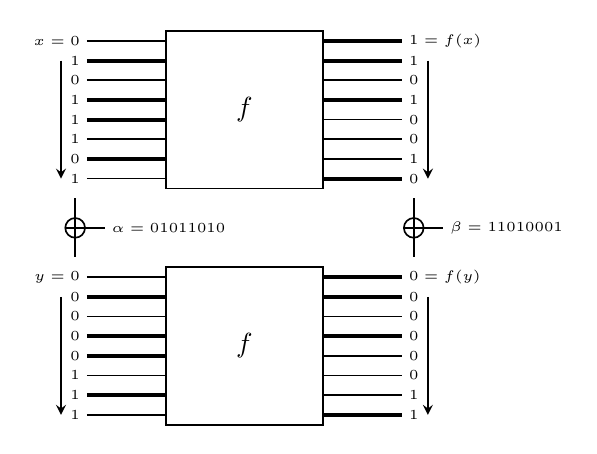
\begin{tikzpicture}[>=stealth, semithick]
            \def\off{0.125}
            \def\step{0.25}
            \tiny
            \newcommand{\normalline}[3]{
                \draw (#1, #2) -- (#1+1, #2) node[left, pos=0] {#3};
            }
            \newcommand{\boldline}[3]{
                \draw[line width=0.5mm] (#1, #2) -- (#1+1, #2);
                \node[left] at (#1, #2) {#3};
            }
            \draw (0, 0) rectangle (2, -2) node[pos=0.5] {\normalsize \(f\)};
            \normalline{-1}{-0*\step-\off}{\(x=0\)}
            \boldline  {-1}{-1*\step-\off}{\(1\)}
            \normalline{-1}{-2*\step-\off}{\(0\)}
            \boldline  {-1}{-3*\step-\off}{\(1\)}
            \boldline  {-1}{-4*\step-\off}{\(1\)}
            \normalline{-1}{-5*\step-\off}{\(1\)}
            \boldline  {-1}{-6*\step-\off}{\(0\)}
            \normalline{-1}{-7*\step-\off}{\(1\)}
            \draw[->] (-1.33, -1*\step-\off) -- (-1.33, -7*\step-\off);
            \normalline{-1}{-0*\step-\off-3}{\(y=0\)}
            \boldline  {-1}{-1*\step-\off-3}{\(0\)}
            \normalline{-1}{-2*\step-\off-3}{\(0\)}
            \boldline  {-1}{-3*\step-\off-3}{\(0\)}
            \boldline  {-1}{-4*\step-\off-3}{\(0\)}
            \normalline{-1}{-5*\step-\off-3}{\(1\)}
            \boldline  {-1}{-6*\step-\off-3}{\(1\)}
            \normalline{-1}{-7*\step-\off-3}{\(1\)}
            \draw[->] (-1.33, -1*\step-\off-3) -- (-1.33, -7*\step-\off-3);

            \renewcommand{\normalline}[3]{
                \draw (#1, #2) -- (#1-1, #2) node[right, pos=0] {#3};
            }
            \renewcommand{\boldline}[3]{
                \draw[line width=0.5mm] (#1, #2) -- (#1-1, #2);
                \node[right] at (#1, #2) {#3};
            }
            \draw (0, -3) rectangle (2, -5) node[pos=0.5] {\normalsize \(f\)};
            \boldline  {3}{-0*\step-\off}{\(1=f(x)\)}
            \boldline  {3}{-1*\step-\off}{\(1\)}
            \normalline{3}{-2*\step-\off}{\(0\)}
            \boldline  {3}{-3*\step-\off}{\(1\)}
            \normalline{3}{-4*\step-\off}{\(0\)}
            \normalline{3}{-5*\step-\off}{\(0\)}
            \normalline{3}{-6*\step-\off}{\(1\)}
            \boldline  {3}{-7*\step-\off}{\(0\)}
            \draw[->] (3.33, -1*\step-\off) -- (3.33, -7*\step-\off);
            \boldline  {3}{-0*\step-\off-3}{\(0=f(y)\)}
            \boldline  {3}{-1*\step-\off-3}{\(0\)}
            \normalline{3}{-2*\step-\off-3}{\(0\)}
            \boldline  {3}{-3*\step-\off-3}{\(0\)}
            \normalline{3}{-4*\step-\off-3}{\(0\)}
            \normalline{3}{-5*\step-\off-3}{\(0\)}
            \normalline{3}{-6*\step-\off-3}{\(1\)}
            \boldline  {3}{-7*\step-\off-3}{\(1\)}
            \draw[->] (3.33, -1*\step-\off-3) -- (3.33, -7*\step-\off-3);

            \draw (-1.15, -8*\step-\off) -- (-1.15, -9*\step-\off);
            \draw (-1.15, -9.5*\step-\off) circle (0.5*\step);
            \draw (-1.15-0.5*\step, -9.5*\step-\off) -- (-1.15+0.5*\step, -9.5*\step-\off);
            \draw (-1.15, -9.5*\step-\off-0.5*\step) -- (-1.15, -9.5*\step-\off+0.5*\step);
            \draw (-1.15, -10*\step-\off) -- (-1.15, -11*\step-\off);
            \draw (-1.15+0.5*\step, -9.5*\step-\off) -- (-1.15+1.5*\step, -9.5*\step-\off) node[right] {\(\alpha = 01011010\)};

            \draw (3.15, -8*\step-\off) -- (3.15, -9*\step-\off);
            \draw (3.15, -9.5*\step-\off) circle (0.5*\step);
            \draw (3.15-0.5*\step, -9.5*\step-\off) -- (3.15+0.5*\step, -9.5*\step-\off);
            \draw (3.15, -9.5*\step-\off-0.5*\step) -- (3.15, -9.5*\step-\off+0.5*\step);
            \draw (3.15, -10*\step-\off) -- (3.15, -11*\step-\off);
            \draw (3.15+0.5*\step, -9.5*\step-\off) -- (3.15+1.5*\step, -9.5*\step-\off) node[right] {\(\beta = 11010001\)};
        \end{tikzpicture}
        \caption{Representation of the differential behaviour of a function \(f\) on a byte, i.e. with \(n = m = 8\). In each drawing of the byte strings, the most significant byte is on top. Since \(x\) and \(y\) are chosen with \(x \oplus y = \alpha\), this diagram occurs with probability \(p\).}
        \label{fig:differential_characteristics}
    \end{figure}
    
    Using differential characteristics, one can formulate the following general strategy for attacking a general cipher.

    {\centering\begin{minipage}{\linewidth}
        \vspace{-0.25cm}
        \begin{algorithm}[H]
            \caption{\textsc{General Differential Attack using Characteristics}}
            \label{algo:general_differential_attack_using_characteristics}
            \begin{algorithmic}[1]
                \Require A function \(E\colon \{0, 1\}^n \times \{0, 1\}^k \to \{0, 1\}^m\), \(k \in \mathbb{N}_{\geq 1}\), with a characteristic \(\alpha \to_p^{E(\cdot, \hat{k})} \beta\) to an unknown key \(\hat{k}\) and \(p \gg 0\).
                \Ensure A candidate for \(\hat{k}\).
                \State Choose pairs \((x_1, y_1), ..., (x_{n_1}, y_{n_1}) \in \{0, 1\}^{2n}\), \(n_1 \in \mathbb{N}_{\geq 1}\), with \(x_i \oplus y_i = \alpha \, \forall \, i \in [1, n]_{\mathbb{N}}\).
                \State Choose keys \(k_1, ..., k_{n_2} \in \{0, 1\}^k\), \(n_2 \in \mathbb{N}_{\geq 1}\), and count \(e_{k_i} \coloneqq |\{(x_j,y_j) \mid E(x_j, k_i) \oplus E(y_j, k_i) = E(x_j, k) \oplus E(y_j, k) = \beta\}|\) for each \(i \in [1, n_2]_{\mathbb{N}}\).
                \State \Return \(k_d\), where \(d \coloneqq \arg\max_{i \in [1, n_2]_{\mathbb{N}}} e_{k_i}\).
            \end{algorithmic}
        \end{algorithm}
    \end{minipage}\par}

    \phantom{}

    This attack relies on replicating the differential behavior of \(E(\cdot, k)\) wrt. \(\alpha \to_p^{E(\cdot, k)} \beta\) as close as possible, it is very loosely formulated and the effectiveness depends on how the choice of the key affects the differential behavior of the cipher as well.
    
    A different approach is to build more sophisticated structures of multiple characteristics, such as \emph{quartets}, which are differential structures of four texts, not just pairs. In the following, we shall demonstrate the \emph{boomerang} attack, following \cite[pp. 162-164]{Knudsen}. Suppose a cipher \(E = E_1 \circ E_0\colon \{0, 1\}^n \to \{0, 1\}^n\) of invertible functions \(E_0, E_1\colon \{0, 1\}^n \to \{0, 1\}^n\) is given. We do not directly consider the key here. Denote \(D_1 \coloneqq E_1^{-1}\) and \(D_0 \coloneqq E_0^{-1}\). Suppose we have the characteristics
    \begin{align}
        \alpha \overunderset{E_0}{p}{\to} \beta, \gamma \overunderset{D_1}{q}{\to} \delta, \beta \overunderset{D_0}{p'}{\to} \alpha
    \end{align}
    where \(p = p'\) may not necessarily hold by definition. The chosen plaintext-ciphertext attack is then performed the following way, following along \Cref{fig:boomerang_attack}:
    \begin{enumerate}[wide]
        \item[\textcolor{orange}{1.}] Choose \(m_0 \in \{0, 1\}^n\) and set \(m_1 \coloneqq m_0 \oplus \alpha\).
        \item[\textcolor{teal}{2.}] Encrypt \(m_0\) and \(m_1\) to obtain ciphertexts \(c_0\) and \(c_1\), store \(u_0\) and \(u_1\). Set \(c_2 \coloneqq c_0 \oplus \gamma\) and \(c_3 \coloneqq c_1 \oplus \gamma\).
        \item[\textcolor{violet}{3.}] Compute \(u_2, u_3\). We have \(\text{Pr}(\bigoplus_{i=0}^3 u_i = 0) \geq q^2\).
        \item[\textcolor{cyan}{4.}] Since \(u_0 \oplus u_1 = \beta\) with probability \(p\), we have \(\text{Pr}(u_2 \oplus u_3 = \beta) \geq pq^2\), giving \(\text{Pr}(m_2 \oplus m_3 = \alpha) = \text{Pr}(\bigoplus_{i=0}^3 m_i = 0) \geq pp'q^2\).
    \end{enumerate}

    \begin{figure}[!hbtp]
        \centering
        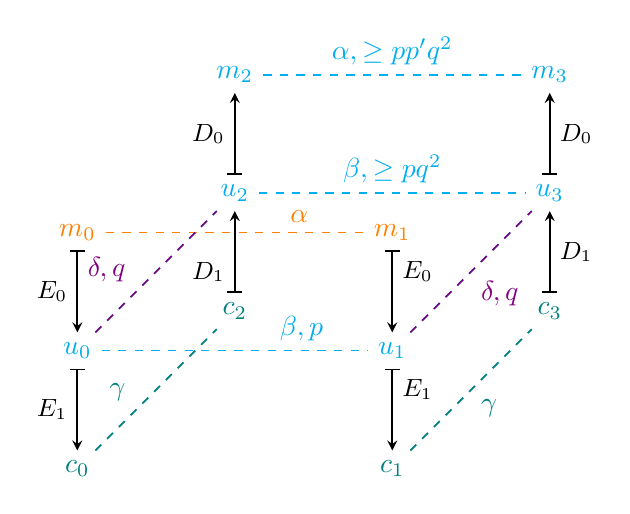
\begin{tikzpicture}[>=stealth, scale=2, semithick]
            \node[orange] (m0) at ($(0, 0)+0*(0, -0.75)$) {\(m_0\)};
            \node[orange] (m1) at ($(2, 0)+0*(0, -0.75)$) {\(m_1\)};
            \node[cyan] (m2) at ($(1, 1)+0*(0, -0.75)$) {\(m_2\)};
            \node[cyan] (m3) at ($(3, 1)+0*(0, -0.75)$) {\(m_3\)};
            \node[cyan] (u0) at ($(0, 0)+1*(0, -0.75)$) {\(u_0\)};
            \node[cyan] (u1) at ($(2, 0)+1*(0, -0.75)$) {\(u_1\)};
            \node[cyan] (u2) at ($(1, 1)+1*(0, -0.75)$) {\(u_2\)};
            \node[cyan] (u3) at ($(3, 1)+1*(0, -0.75)$) {\(u_3\)};
            \node[teal] (c0) at ($(0, 0)+2*(0, -0.75)$) {\(c_0\)};
            \node[teal] (c1) at ($(2, 0)+2*(0, -0.75)$) {\(c_1\)};
            \node[teal] (c2) at ($(1, 1)+2*(0, -0.75)$) {\(c_2\)};
            \node[teal] (c3) at ($(3, 1)+2*(0, -0.75)$) {\(c_3\)};
            \path[|->]
                (m0) edge node[left,  pos=0.5] {\small \(E_0\)}    (u0)
                (u0) edge node[left,  pos=0.5] {\small \(E_1\)}    (c0)
                (m1) edge node[above right, pos=0.5] {\small \(E_0\)}    (u1)
                (u1) edge node[above right, pos=0.5] {\small \(E_1\)}    (c1)
                (u2) edge node[left,  pos=0.5] {\small \(D_0\)}    (m2)
                (c2) edge node[below left,  pos=0.5] {\small \(D_1\)} (u2)
                (u3) edge node[right, pos=0.5] {\small \(D_0\)}    (m3)
                (c3) edge node[right, pos=0.5] {\small \(D_1\)} (u3)
            ;
            \path
                (m0) edge[dashed, orange] node[above, pos=0.75, orange] {\(\alpha\)} (m1)
                (c0) edge[dashed, teal] node[above left, teal, pos=0.33] {\(\gamma\)} (c2)
                (c1) edge[dashed, teal] node[below right, teal, pos=0.5] {\(\gamma\)} (c3)
                (u0) edge[dashed, cyan] node[above, pos=0.75, cyan] {\(\beta, p\)} (u1)
                (u0) edge[dashed, cyan] (u2)
                (u1) edge[dashed, cyan] (u3)
                (u2) edge[dashed, cyan] node[above, pos=0.5, cyan] {\(\beta, \geq pq^2\)} (u3)
                (u0) edge[dashed, violet] node[above left, violet, pos=0.33] {\(\delta, q\)} (u2)
                (u1) edge[dashed, violet] node[below right, violet, pos=0.5] {\(\delta, q\)} (u3)
                (m2) edge[dashed, cyan] node[above, pos=0.5, cyan] {\(\alpha, \geq pp'q^2\)} (m3)
            ;
        \end{tikzpicture}
        \caption{The general Boomerang attack.}
        \label{fig:boomerang_attack}
    \end{figure}

    The condition \(\bigoplus_{i=0}^3 m_i\) can then be used for attacking the key, see \cite[pp. 161-162]{Wagner_1999} for an example. The crucial condition for success here is whether \(pp'q^2 \gg 0\).
    
    The boomerang attack can be improved to only a chosen ciphertext attack with more available plaintexts, yielding the \emph{amplified boomerang} and \emph{rectangle} attacks \cite[pp. 164-165]{Knudsen}. The main conclusion to draw from this section is, that highly probable differential characteristics are crucial for successful attacks by differential cryptanalysis, as directly shown e.g. in the cryptanalysis of COCONUT98, where a precise analysis of the Feistel block cipher structure yielded a characteristic of probability \(\approx 1/1900\) using texts with single one-entries each, breaking the cipher \cite[pp. 160-161]{Wagner_1999}. Furthermore, for some current research on quantum boomerang attacks, see \cite{Frixons_2022, Zou_2023}.

    \section{A Hybrid Adiabatic-Gatebased Quantum Attack} Suppose a function \(f\colon \{0, 1\}^n \to \{0, 1\}^m\) is given and our objective is to find one of the highest probable characteristic of it. Denote the oracles
    \begin{align}
        &U_{\oplus}\colon \mathbb{C}^{3N} \to \mathbb{C}^{3N}, \ket{(x, y)}\ket{z} \mapsto \ket{(x, y)}\ket{z \oplus (x \oplus y)}\\
        &U_{f \oplus f \times 0}\colon \mathbb{C}^{3N+M} \to \mathbb{C}^{3N+M}, \ket{(x, y, z)}\ket{a} \mapsto \ket{(x, y, z)}\ket{a \oplus (f(x) \oplus f(y))}
    \end{align}
    Then one may execute the following computations:
    \begin{align}
        \ket{0}^{\otimes (3n+m)} &\xmapsto{H^{\otimes 2n} \otimes E_{2M}} \frac{1}{N} \sum_{x, y \in \{0, 1\}^n} \ket{x}\ket{y}\ket{0}^{\otimes (n+m)} = \frac{1}{N} \sum_{\alpha, x \in \{0, 1\}^n} \ket{x}\ket{x \oplus \alpha}\ket{0}^{\otimes (n+m)}\\
        &\xmapsto{(U_{f \oplus f \times 0}) (U_{\oplus} \otimes E_M)} \frac{1}{N} \sum_{\alpha, x \in \{0, 1\}^n} \ket{x}\ket{x \oplus \alpha}\ket{\alpha}\ket{f(x) \oplus f(x \oplus \alpha)}\\
        &= \frac{1}{N}\sum_{(\alpha, \beta) \in \{0, 1\}^{n+m}} \left(\sum_{x \in \{0, 1\}^n, f(x) \oplus f(x \oplus \alpha) = \beta} \ket{x}\ket{x \oplus \alpha}\right)\ket{\alpha}\ket{\beta}
    \end{align}
    Our objective is to find a difference pair \((\alpha, \beta)\) with the highest number of pairs \((x, x \oplus \alpha)\) which admit to the associated characteristic. That corresponds to the highest probable result when measuring wrt. the observable \(\{\Span(\{\ket{x}\ket{y}\ket{\alpha}\ket{\beta} \mid x, y \in \{0, 1\}^n\}) \mid (\alpha, \beta) \in \{0, 1\}^{n + m}\}\), so the task may be reduced to the problem of finding the highest amplitude of a given state.

    Consider the simplest case: A state \(\ket{\phi} = \sum_{j = 0}^{N-1} \alpha_j \ket{j}\) is given and we want to find \(\arg\max_{j \in \{0, 1\}^n} |\alpha_j|^2\). Our proposal is to use the following adiabatic quantum algorithm. We can observe
    \begin{align}
        \ketbra{\phi}{\phi} = \sum_{j=0}^{N-1} |a_j|^2 \ketbra{j}{j}
    \end{align}
    Thus
    \begin{align}
        H_1 \coloneqq E_N-\ketbra{\phi}{\phi} = \sum_{j=0}^{N-1} (1-|\alpha_j|^2) \ketbra{j}{j}
    \end{align}
    We have \(\sigma(H_1) = \{1 - |\alpha_j|^2 \mid j \in \{0, 1\}^n\}\), thus the problem reduces to find the ground state of the Hamiltonian \(H_1\). We recall the necessary tools for such an adiabatic quantum algorithm: A proper initial Hamiltonian \(H_0\), an appropriate schedule \(A\) and possibly a catalyst Hamiltonian \(A\). Furthermore, one needs to find out how exactly to apply this algorithm to the problem from above, since there are still the first two registers in the state, so an observable encoding function \(\chi\) needs to be given to the algorithm in an appropriate form. Also, of course, the analysis wrt. the rigorous adiabatic theorem must be performed.

    Returning to the problem of finding characteristics, our hybrid adiabatic-gatebased quantum algorithm, in the end, would need to measure wrt. the canonical basis to get the highest probable characteristic differences and then perform amplitude estimation with runtime e.g. \(O(\sqrt{N})\) \cite[pp. 19-20]{Brassard} to approximate its probability, assuming the knowledge of it is needed.

    \section{The Rijndael S-Box Differential Property} A counterexample to the existence of high probability characteristics for any function is the Rijndael S-Box. Recall the following concepts from the Rijndael algorithm: The factor ring \(F \coloneqq \text{GF}(2)[x]/(x^8+x^4+x^3+x+1)\) \cite[pp. 10-11]{Dworkin_2023} is a field \cite[pp. 313-314]{Fischer}, which is bijective to \(\text{GF}(2)^8\) via the uniqueness of polynomial division in a polynomial ring over a field. Thus, we may represent a byte using such a polynomial via the canonical isomorphism of the additive groups. For the description of the Rijndael S-Box following \cite[pp. 15-16]{Dworkin_2023}, we now define the following \emph{patched inverse} and affine linear transformation
    \begin{align}
        \iota\colon F \to F, x \mapsto \begin{cases}
            x^{-1} & x \neq 0\\
            0 & x = 0
        \end{cases} \qquad L_A\coloneqq \begin{pmatrix}
            1 & 0 & 0 & 0 & 1 & 1 & 1 & 1\\
            1 & 1 & 0 & 0 & 0 & 1 & 1 & 1\\
            1 & 1 & 1 & 0 & 0 & 0 & 1 & 1\\
            1 & 1 & 1 & 1 & 0 & 0 & 0 & 1\\
            1 & 1 & 1 & 1 & 1 & 0 & 0 & 0\\
            0 & 1 & 1 & 1 & 1 & 1 & 0 & 0\\
            0 & 0 & 1 & 1 & 1 & 1 & 1 & 0\\
            0 & 0 & 0 & 1 & 1 & 1 & 1 & 1
        \end{pmatrix} \qquad v_A \coloneqq \begin{pmatrix}
            1\\
            1\\
            0\\
            0\\
            0\\
            1\\
            1\\
            0
        \end{pmatrix}
    \end{align}
    from which the S-Box is then defined as
    \begin{align}
        S\colon F \to F, x \mapsto (L \circ \iota)(x)+v_A
    \end{align}
    With \(\oplus\) we shall denote the additive operation of \(\text{GF}(2)^8\), with \(+\) the additive operation of \(F\). The theorem of interest is now the following.
    \begin{theorem}[{AES S-Box Differential Property \cite[pp. 62-63]{Bonnetain_2019}}]
        Let \(\alpha, \beta \in F \setminus \{0\} = F^*\) be arbitrary and loose. The following two statements hold.
        \begin{enumerate}[label=(\roman*), wide] \label{thm:aes_s_box_differential_property}
            \item \label{thm:aes_s_box_differential_property_1} \(S\) possesses the following characteristics:
            \begin{align}
                0 \overunderset{S}{1}{\to} 0, \alpha \overunderset{S}{0}{\to} 0, 0 \overunderset{S}{0}{\to} \beta
            \end{align}
            \item \label{thm:aes_s_box_differential_property_2} The characteristic \(\alpha \to_p^S \beta\) has probability \(p \in \{0, 2^{-7}, 2^{-6}\}\).
        \end{enumerate}
    \end{theorem}

    \begin{proof}
        \begin{enumerate}[wide]
            \item[\ref{thm:aes_s_box_differential_property_1}] Let \(x \in F\) be loose. We consider the equation
            \begin{align}
                S(x) \oplus S(x \oplus \alpha) = \beta \leadsto \iota(x) \oplus \iota(x \oplus \alpha) = L^{-1}(\beta) \eqqcolon \hat{\beta} \label{eq:aes_s_box_differential_property_1}
            \end{align}
            For \(\alpha = \beta = 0\), this reads
            \begin{align}
                \iota(x) \oplus \iota(x) = 0
            \end{align}
            which holds for all \(x \in F\). For \(\alpha \neq 0, \beta = 0\), we have
            \begin{align}
                \iota(x) \oplus \iota(x \oplus \alpha) = 0 \leadsto \iota(x) = \iota(x \oplus \alpha)
            \end{align}
            \(0 = 0\) would imply \(\alpha = 0\), which is wrong \lightning. \(x = 0\) or \(x = \alpha\) is also not possible. \(x^{-1} = (x \oplus \alpha)^{-1}\) gives \(\alpha = 0\), which is also false. For \(\alpha = 0, \beta \neq 0\), we get
            \begin{align}
                0 = \hat{\beta}
            \end{align}
            which is false, as \(\text{ker}(L^{-1}) = \{0\}\).
            \item[\ref{thm:aes_s_box_differential_property_2}] We continue using \Cref{eq:aes_s_box_differential_property_1}. We first consider the case \(x(x \oplus \alpha) = 0\). Wlog. we consider \(x = 0\), as the case \(x = \alpha\) is dual. We thus have \(\alpha = \hat{\beta}^{-1}\), so we may consider the probability \(p\) of the characteristic \(\alpha \to_p^S L(\alpha^{-1})\). The condition gives
            \begin{align}
                \iota(x) \oplus \iota(x \oplus \alpha) = \alpha^{-1}
            \end{align}
            \(x = 0\) and \(x = \alpha\) suffice the condition. Else we have
            \begin{align}
                (x \oplus \alpha)^{-1} = x^{-1} \oplus \alpha^{-1} \leadsto x^2 \oplus \alpha x \oplus \alpha^2 = 0 \leadsto (x/\alpha)^2 \oplus x/\alpha \oplus 1 = 0
            \end{align}
            Substituting \(\hat{x} \coloneqq x/\alpha\), we reduce this problem to \(\hat{x}^2 \oplus \hat{x} \oplus 1 = 0\) over \(F\). This has either no or two solutions, totalling two to four, giving the claim.
            
            Now we look at the case \(x(x \oplus \alpha) \neq 0\). There we have
            \begin{align}
                x^{-1} \oplus (x \oplus \alpha)^{-1} = \hat{\beta} \leadsto x^2 \oplus \alpha x \oplus \alpha \hat{\beta}^{-1} = 0
            \end{align}
            Rewriting the equation as \((x/\alpha)^2 \oplus x/\alpha \oplus \hat{\beta}^{-1}/\alpha\), we may use a quantum algorithm for determining a solution of an equation of form \(x^2 \oplus x \oplus d = 0\) \cite[pp. 64-65]{Bonnetain_2019}. The details shall be omitted here. This yields two solutions.
        \end{enumerate}
    \end{proof}

    \Cref{thm:aes_s_box_differential_property} \ref{thm:aes_s_box_differential_property_2} gives, that the Rijndael S-Box has characteristics of comparatively low probability for non-trivial characteristics, even though \(2^{-7}\) and \(2^{-6}\) are still high enough complexities for cryptanalysis by computer, omitting at this point that the S-Box on its own is invertible, of course. The more important question that arises is how this can be used for the cryptanalysis of AES, which is considered as secure against differential cryptanalysis, and how this fact is connected with the rest of the algorithm. For more information see \cite{Bonnetain_2019}.

    \printbibliography{}
\end{document}
